\eventsection{RESULTADOS E DISCUSS\~AO}

A Tabela \ref{tab:metricas} apresenta a s\'intese quantitativa dos resultados no conjunto de teste temporal. O LightGBM obteve o melhor desempenho global, com menor erro absoluto na regress\~ao e superioridade nas principais m\'etricas de classifica\c{c}\~ao. Esse resultado indica que, no cen\'ario avaliado, a estrat\'egia de \textit{boosting} foi mais eficaz para discriminar surtos raros do que a abordagem baseada em \textit{bagging}.

\begin{table}[H]
\centering
\caption{Desempenho comparativo dos modelos no conjunto de teste.}
\label{tab:metricas}
\tabelafonte
\begin{tabular}{lcccccc}
\toprule
Modelo & MAE & RMSE & AUC-ROC & AUC-PR & Brier & F1 \\
\midrule
LightGBM & 31,90 & 60,54 & 0,892 & 0,674 & 0,053 & 0,397 \\
XGBoost & 35,82 & 67,33 & 0,827 & 0,412 & 0,067 & 0,364 \\
Random Forest & 34,08 & 63,01 & 0,778 & 0,348 & 0,077 & 0,273 \\
\bottomrule
\end{tabular}
\artigofonte{elabora\c{c}\~ao pr\'opria a partir dos relat\'orios experimentais.}
\end{table}

Os resultados refor\c{c}am dois pontos principais. Primeiro, a din\^amica recente da s\'erie epidemiol\'ogica foi o sinal mais relevante para a distin\c{c}\~ao entre surto e n\~ao surto. Segundo, vari\'aveis clim\'aticas n\~ao se mostraram suficientes de forma isolada, mas agregaram valor quando combinadas aos atributos epidemiol\'ogicos. Esse comportamento \'e coerente com a literatura que descreve a transmiss\~ao de mal\'aria como fen\^omeno dependente de m\'ultiplos fatores ambientais e temporais \cite{arisco2025impact}.

Em rela\c{c}\~ao aos trabalhos j\'a citados, a principal contribui\c{c}\~ao deste artigo n\~ao est\'a na cria\c{c}\~ao de um novo algoritmo, mas na organiza\c{c}\~ao de um protocolo comparativo aplicado ao contexto amaz\^onico com foco expl\'icito em detec\c{c}\~ao de surtos. Enquanto \citeonline{monteiro2025integrating} enfatizam previs\~ao de casos com integra\c{c}\~ao espacial, aqui o foco recai sobre classifica\c{c}\~ao operacional de eventos raros com separa\c{c}\~ao temporal estrita. Em contraste com revis\~oes amplas sobre desbalanceamento \cite{5128907,branco2015surveypredictivemodellingimbalanced,johnson2019survey}, o presente estudo mostra como essas recomenda\c{c}\~oes se comportam em uma base epidemiol\'ogica real, com depend\^encia temporal, baixa preval\^encia e necessidade de uso em vigil\^ancia.

Em leitura conjunta das m\'etricas, o LightGBM se destacou nas duas frentes avaliadas. Em regress\~ao, produziu o menor erro absoluto m\'edio. Em classifica\c{c}\~ao, concentrou simultaneamente a melhor AUC-ROC, a melhor AUC-PR e o menor \textit{Brier Score}. Isso indica vantagem n\~ao apenas em discrimina\c{c}\~ao global, mas tamb\'em em ordena\c{c}\~ao probabil\'istica, aspecto central quando o objetivo \'e produzir alerta de risco e n\~ao apenas r\'otulos bin\'arios.

Esse padr\~ao \'e consistente com a literatura que recomenda priorizar curvas Precision-Recall e medidas de calibra\c{c}\~ao em classes raras, em vez de indicadores agregados simplificados \cite{saito2015precision,davis2006relationship}. Assim, o artigo n\~ao apenas confirma um vencedor entre os modelos comparados, mas demonstra por que essa vantagem \'e relevante para uma decis\~ao aplicada em sa\'ude p\'ublica.

Do ponto de vista operacional, o contraste entre os modelos aparece com clareza nas matrizes de confus\~ao. No teste temporal, o XGBoost detectou 20 dos 28 surtos, com 8 falsos negativos e 62 falsos positivos. O LightGBM detectou 23 surtos, com apenas 5 falsos negativos e 65 falsos positivos. J\'a o Random Forest detectou 22 surtos, por\'em gerou 111 falsos positivos, o que reduz sua utilidade em rotinas de vigil\^ancia por elevar a carga de verifica\c{c}\~ao sobre eventos n\~ao confirmados.

\begin{figure}[!htb]
\centering
\caption{Matrizes de confus\~ao dos modelos avaliados no conjunto de teste temporal.}
\label{fig:confusoes}
\begin{subfigure}[t]{0.47\textwidth}
\centering
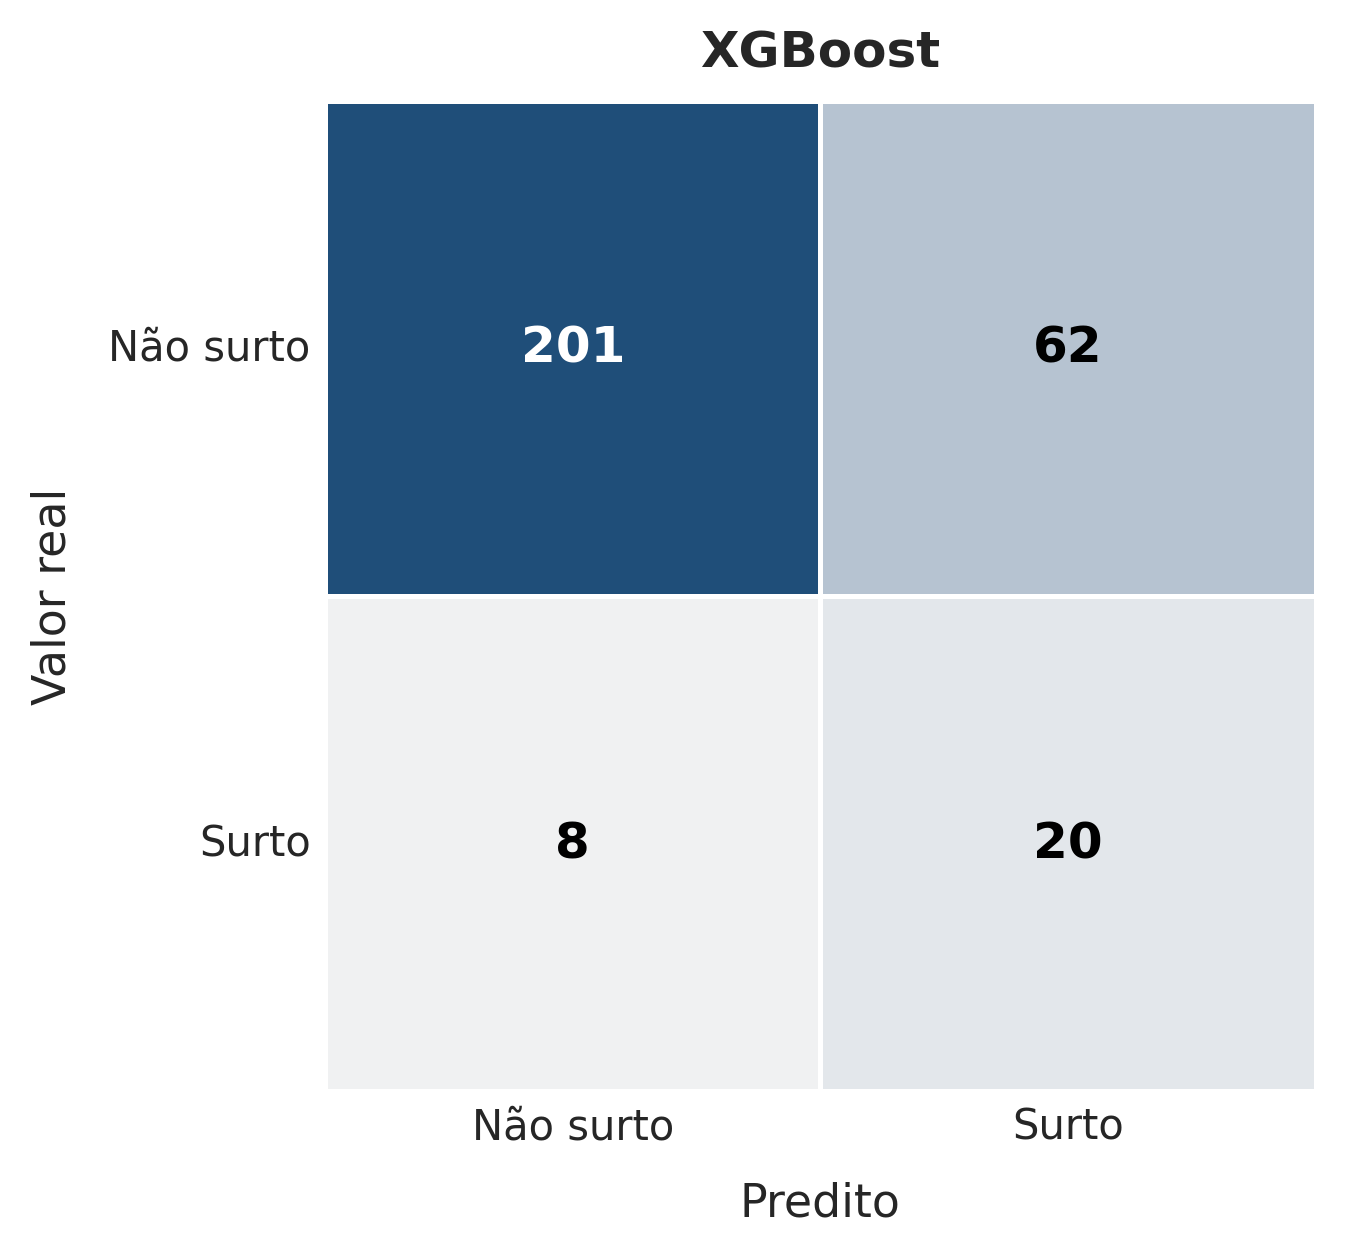
\includegraphics[width=\textwidth]{figs/confusion_clean/xgb_clean.png}
\caption{XGBoost}
\label{fig:confusao-xgb}
\end{subfigure}
\hfill
\begin{subfigure}[t]{0.47\textwidth}
\centering
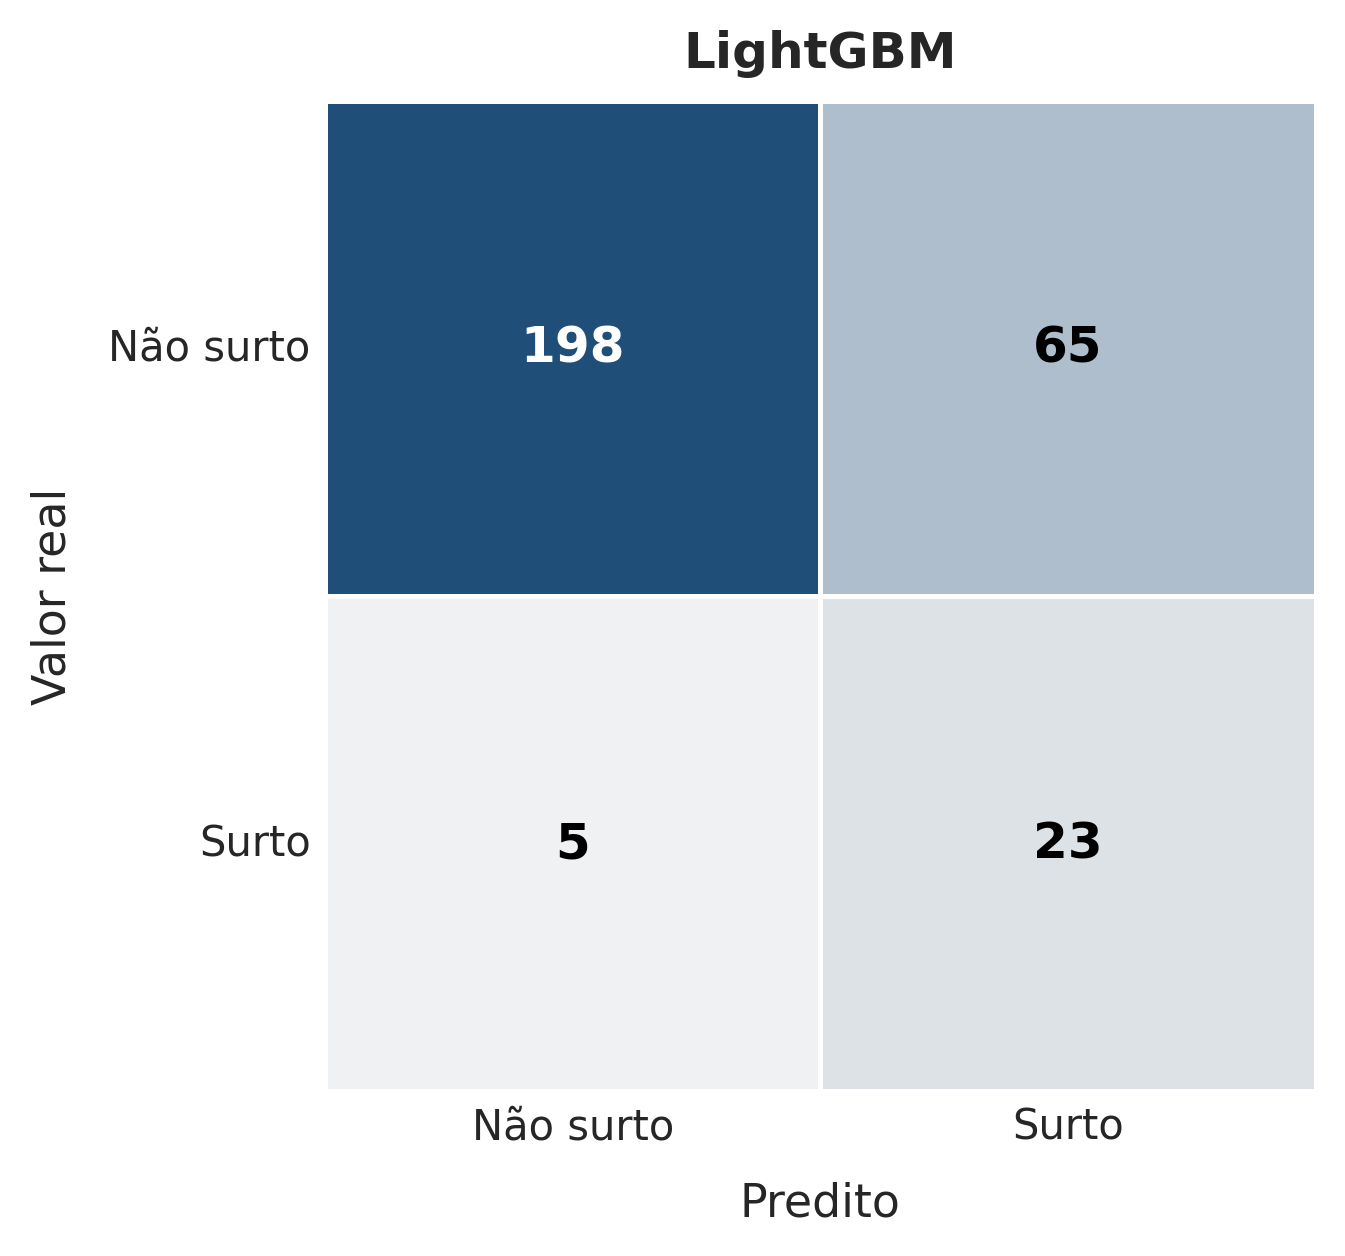
\includegraphics[width=\textwidth]{figs/confusion_clean/lgbm_clean.png}
\caption{LightGBM}
\label{fig:confusao-lgbm}
\end{subfigure}

\vspace{0.6cm}

\begin{subfigure}[t]{0.47\textwidth}
\centering
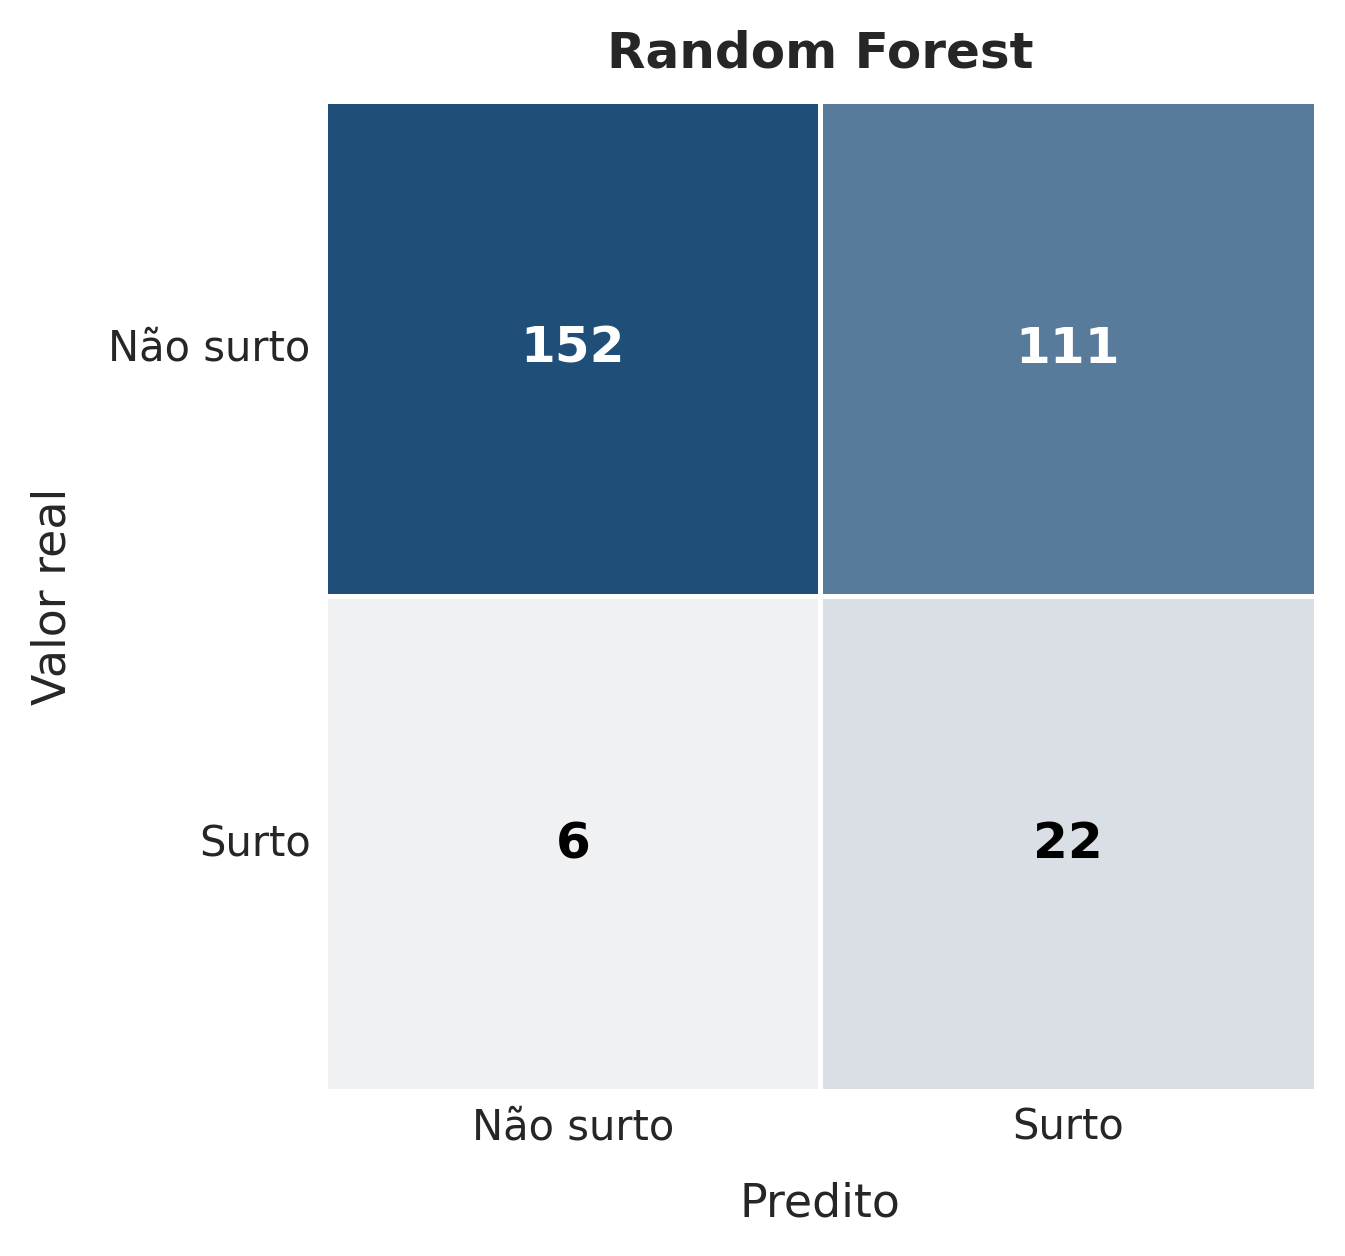
\includegraphics[width=\textwidth]{figs/confusion_clean/rf_clean.png}
\caption{Random Forest}
\label{fig:confusao-rf}
\end{subfigure}
\artigofonte{elabora\c{c}\~ao pr\'opria.}
\end{figure}

A Figura \ref{fig:confusoes} mostra que o ganho do LightGBM n\~ao decorre apenas de maior sensibilidade, mas de melhor equil\'ibrio entre recupera\c{c}\~ao de surtos e estabilidade probabil\'istica. Esse padr\~ao \'e compat\'ivel com os valores de AUC-PR e \textit{Brier Score}, que favorecem o LightGBM em rela\c{c}\~ao aos demais modelos.

Do ponto de vista interpretativo, isso explicita uma diferen\c{c}a importante frente a compara\c{c}\~oes mais gen\'ericas de algoritmos: neste trabalho, a utilidade do modelo \'e analisada tamb\'em pelo custo operacional de falsos alertas. Esse enquadramento aproxima a avalia\c{c}\~ao do cen\'ario concreto da vigil\^ancia epidemiol\'ogica.

\eventsubsection{An\'alise complementar}

A an\'alise de import\^ancia de atributos mostrou converg\^encia parcial entre os modelos. O atributo \texttt{casos\_novos\_malaria\_trend} apareceu como principal preditor nos tr\^es algoritmos, indicando que a din\^amica recente da s\'erie epidemiol\'ogica concentra a maior parte do sinal para discrimina\c{c}\~ao de surtos. Nos modelos de \textit{boosting}, vari\'aveis clim\'aticas e de intera\c{c}\~ao tamb\'em tiveram participa\c{c}\~ao relevante, o que sugere complementaridade entre hist\'orico epidemiol\'ogico e sazonalidade ambiental.

\begin{table}[H]
\centering
\caption{Principais atributos para classifica\c{c}\~ao de surto por modelo.}
\label{tab:atributos}
\tabelafonte
\begin{tabular}{lll}
\toprule
Posi\c{c}\~ao & XGBoost & LightGBM \\
\midrule
1 & \texttt{casos\_novos\_malaria\_trend} & \texttt{casos\_novos\_malaria\_trend} \\
2 & \texttt{dias\_com\_chuva\_lag3} & \texttt{temp\_x\_casos\_ma3} \\
3 & \texttt{chuva\_total\_mes\_ma3} & \texttt{casos\_novos\_malaria\_ma6} \\
4 & \texttt{umid\_media\_mes\_ma3} & \texttt{temp\_max\_media\_mes\_ma6} \\
5 & \texttt{temp\_media\_mes} & \texttt{casos\_novos\_malaria\_ma3} \\
\bottomrule
\end{tabular}
\artigofonte{elabora\c{c}\~ao pr\'opria com base nos relat\'orios de import\^ancia de atributos.}
\end{table}

Os testes de abla\c{c}\~ao e de robustez temporal refor\c{c}aram essa interpreta\c{c}\~ao. O uso isolado de vari\'aveis clim\'aticas gerou desempenho fraco, enquanto o bloco epidemiol\'ogico preservou parte relevante da capacidade discriminativa. Quando as duas fontes de informa\c{c}\~ao foram combinadas, o desempenho melhorou de modo consistente. Em termos temporais, o LightGBM manteve ordena\c{c}\~ao probabil\'istica \'util mesmo quando avaliado por ano, embora com oscila\c{c}\~ao do F1 conforme o regime epidemiol\'ogico.

Esse resultado refor\c{c}a outra contribui\c{c}\~ao do estudo: mostrar que a superioridade do modelo n\~ao depende exclusivamente de um recorte agregado de teste, mas se preserva de forma razo\'avel quando o problema \'e reobservado sob varia\c{c}\~ao anual e sob redefini\c{c}\~oes operacionais do alvo.

\begin{table}[H]
\centering
\caption{Resumo de abla\c{c}\~ao, robustez temporal e sensibilidade do alvo.}
\label{tab:ablation}
\tabelafonte
\begin{tabular}{lcccc}
\toprule
Cen\'ario & ROC-AUC & PR-AUC & F1 & Brier \\
\midrule
Completo & 0,864 & 0,536 & 0,489 & 0,067 \\
Sem intera\c{c}\~oes & 0,872 & 0,568 & 0,508 & 0,061 \\
Epidemiol\'ogico apenas & 0,804 & 0,352 & 0,491 & 0,091 \\
Clim\'atico apenas & 0,563 & 0,210 & 0,205 & 0,108 \\
Clima + epidemiologia & 0,873 & 0,569 & 0,508 & 0,060 \\
\midrule
Robustez 2023 & 0,714 & 0,469 & 0,444 & 0,069 \\
Robustez 2024 & 0,862 & 0,630 & 0,375 & 0,054 \\
Robustez 2025 & 0,878 & 0,415 & 0,218 & 0,080 \\
\midrule
Quantil 0,85 & 0,764 & 0,339 & -- & 0,115 \\
Quantil 0,90 & 0,704 & 0,380 & -- & 0,099 \\
Quantil 0,95 & 0,767 & 0,281 & -- & 0,053 \\
\bottomrule
\end{tabular}
\artigofonte{elabora\c{c}\~ao pr\'opria a partir dos relat\'orios de abla\c{c}\~ao, robustez temporal e valida\c{c}\~ao adicional.}
\end{table}

Os valores da Tabela \ref{tab:ablation} indicam que o modelo n\~ao depende exclusivamente das vari\'aveis clim\'aticas, mas tamb\'em n\~ao se sustenta apenas sobre uma l\'ogica ambiental simplificada. A melhor resposta emerge da combina\c{c}\~ao entre clima e hist\'orico recente de casos. Al\'em disso, a sensibilidade a diferentes quantis de defini\c{c}\~ao de surto mostrou queda moderada, e n\~ao colapso, o que \'e um sinal importante de estabilidade conceitual do pipeline.

Em termos interpretativos, os achados sustentam a ado\c{c}\~ao de modelos de \textit{boosting} em sistemas de alerta epidemiol\'ogico para mal\'aria no Amazonas, especialmente quando o objetivo \'e priorizar eventos raros com depend\^encia temporal. Ainda assim, alguns limites precisam ser considerados. O estudo permanece restrito ao Amazonas, a defini\c{c}\~ao de surto foi operacionalizada por quantil municipal e o n\'umero absoluto de eventos positivos no teste ainda \'e relativamente pequeno. Portanto, embora os resultados sejam consistentes, a generaliza\c{c}\~ao para outros contextos exige valida\c{c}\~ao adicional.

Essa delimita\c{c}\~ao tamb\'em ajuda a posicionar corretamente o alcance do artigo. A contribui\c{c}\~ao aqui produzida \'e uma evid\^encia aplicada, metodologicamente rigorosa e contextualizada para a Amaz\^onia, e n\~ao uma afirma\c{c}\~ao universal sobre superioridade de um algoritmo em qualquer cen\'ario epidemiol\'ogico.

Do ponto de vista de governan\c{c}a e reprodutibilidade, a arquitetura do pipeline foi mantida modular, com separa\c{c}\~ao clara entre pr\'e-processamento, treinamento e gera\c{c}\~ao de relat\'orios. Essa organiza\c{c}\~ao facilita auditoria, reexecu\c{c}\~ao e atualiza\c{c}\~ao por novas janelas temporais. O fluxo tamb\'em tolera execu\c{c}\~ao heterog\^enea, com acelera\c{c}\~ao por GPU quando dispon\'ivel e alternativa est\'avel em CPU, sem alterar o protocolo metodol\'ogico. Em cen\'arios de uso real, recomenda-se complementar o modelo com monitoramento de deriva, recalibra\c{c}\~ao de limiares e rastreabilidade de vers\~oes, em sintonia com recomenda\c{c}\~oes de governan\c{c}a para IA em sa\'ude \cite{world2024ethics}.
